\documentclass[11pt]{article}
\usepackage{amsfonts} 
\usepackage{amsmath}
\usepackage{graphicx}
\usepackage{listings}
\usepackage{float}
\usepackage{hyperref}
\usepackage{wrapfig}%
\usepackage{xcolor}

\definecolor{codegreen}{rgb}{0,0.6,0}
\definecolor{codegray}{rgb}{0.5,0.5,0.5}
\definecolor{codepurple}{rgb}{0.58,0,0.82}
\definecolor{backcolour}{rgb}{0.95,0.95,0.92}

\lstdefinestyle{mystyle}{
    backgroundcolor=\color{backcolour},   
    commentstyle=\color{codegreen},
    keywordstyle=\color{magenta},
    numberstyle=\tiny\color{codegray},
    stringstyle=\color{codepurple},
    basicstyle=\ttfamily\footnotesize,
    breakatwhitespace=false,         
    breaklines=true,                 
    captionpos=b,                    
    keepspaces=true,                 
    numbers=left,                    
    numbersep=5pt,                  
    showspaces=false,                
    showstringspaces=false,
    showtabs=false,                  
    tabsize=2
}

\lstset{style=mystyle}

\begin{document}

{\centering
  \large Solution for the Second Joint Assignment (part 2)\\
   Danis Alukaev BS19-02\\ \par
}

\bigbreak
\noindent $\textbf{2.1. Plot the graph of a point cloud and regression polynomial.}$\\

\noindent Given $n$ points on a 2D plane $(x_{1},y_{1}), (x_{2},y_{2}), ...,(x_{n},y_{n})$ with $x_{1} < x_{2} < ... < x_{n}$ that lie roughly within the neighbourhood of a parabola. The goal is to approximate this data set with a single parabolic function. Apparently, we have to find such coefficients $a$, $b$ and $c$ of a second degree parabola $y = a + bx + cx^{2}$ that fit given $n$ points with a minimum sum of squared errors $SSE=\sum_{i=1}^{n}(y_{i}-(a + bx_{i}+cx_{i}^{2}))^{2}$. \\

\begin{figure}[h]
\centering
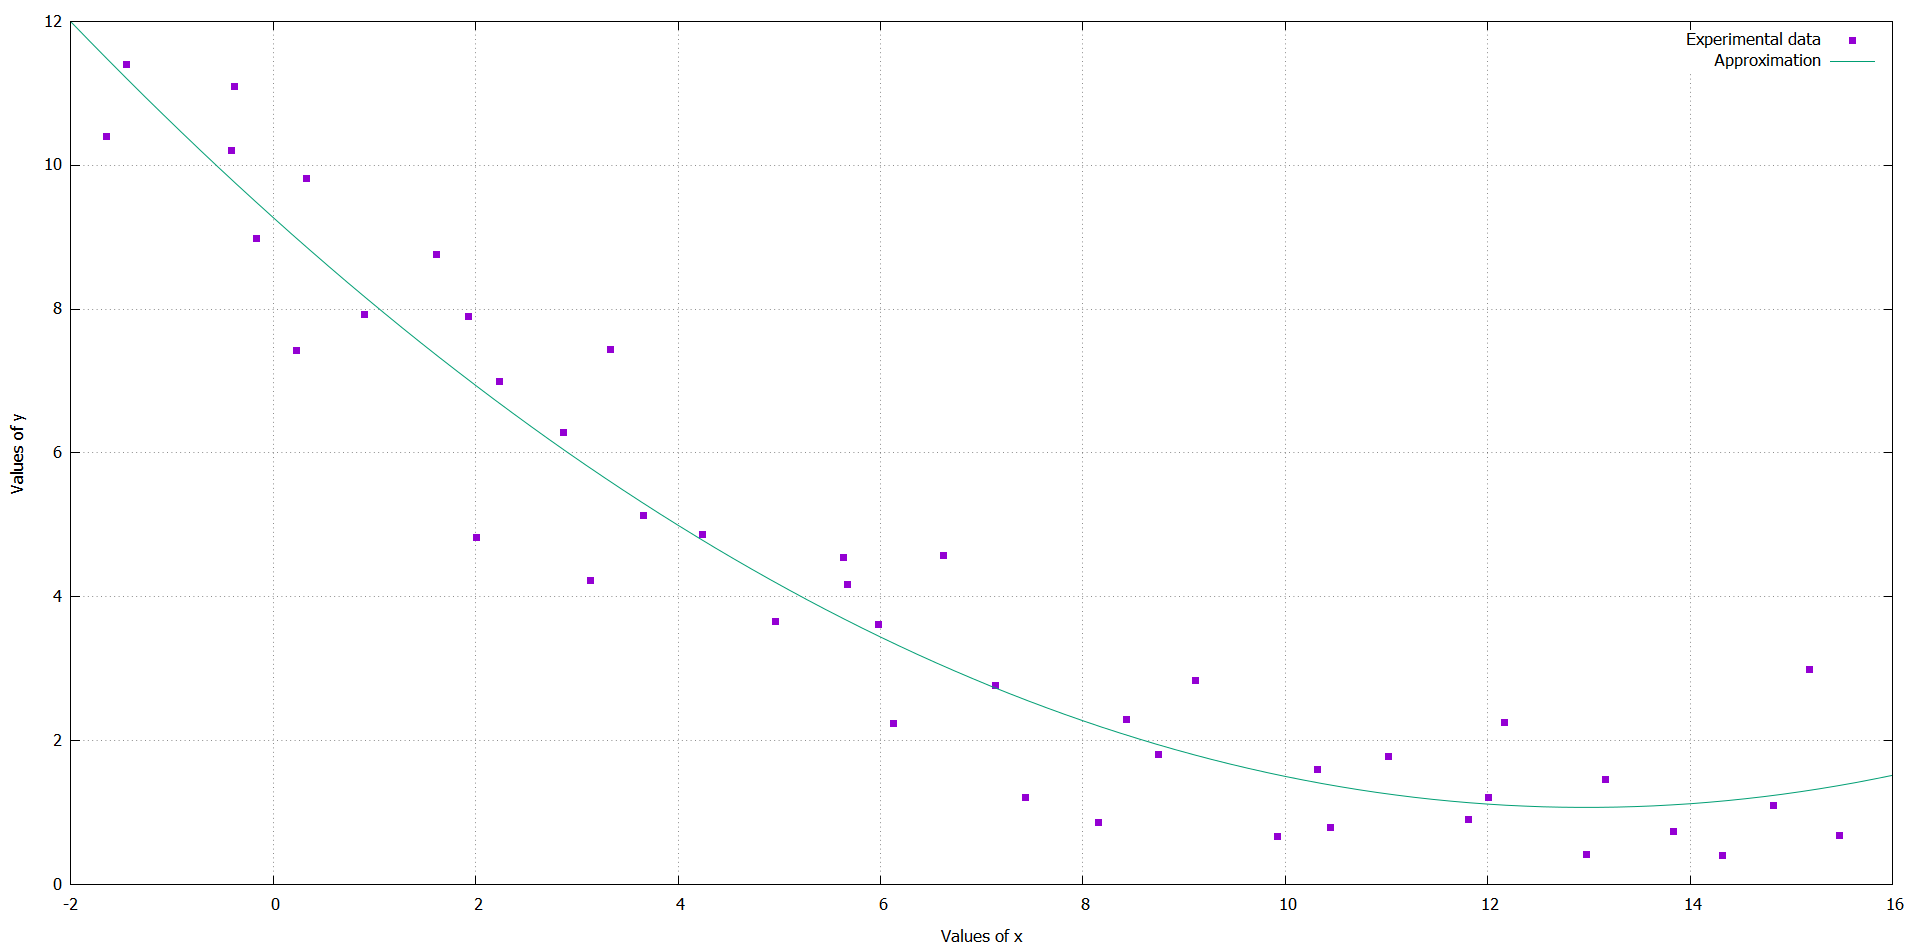
\includegraphics[width=\textwidth]{Least_squares_approximation.png}
\caption{Parabolic least-squares approximation}
\label{fig:mpr}
\end{figure}

\noindent The proposed algorithm (see 2.2 for further details) was evaluated on the following dataset containing 43 points:\\ 
\noindent $\{(-1.645, 10.400), (-1.451, 11.400), (-0.381, 11.100), (-0.411, 10.200),\\
(-0.170, 8.982), (0.232, 7.421), (0.332, 9.821), (0.896, 7.931),(1.613, 8.765),\\ (1.932, 7.893), (2.012, 4.821), (2.237, 6.997),
(2.871, 6.286), (3.137, 4.234),\\ (3.337, 7.434), (3.658, 5.131),
(4.240, 4.871), (4.963, 3.658), (5.632, 4.546),\\ (5.673, 4.169),
(5.981, 3.613), (6.128, 2.245), (6.625, 4.572), (7.132, 2.763),\\
(7.432, 1.213), (8.156, 0.856), (8.432, 2.295), (8.742, 1.802),
(9.113, 2.843),\\ (9.923, 0.662), (10.450, 0.794), (10.323, 1.598),
(11.016, 1.786), (11.813, 0.898), \\ (12.013, 1.214), (12.167, 2.257),
(12.972, 0.416), (13.168, 1.466), (13.834, 0.732),\\ (14.321, 0.401),
(14.821, 1.098), (15.178, 2.987), (15.478, 0.687)\}$, where first entry of the ordered pair is x-coordinate of a particular point, and the second entry is the y-coordinate.\\


\noindent Let $A=\begin{bmatrix}
1 & x_{1} & x_{1}^{2}\\
1 & ... & ...\\
1 & x_{n} & x_{n}^{2}
\end{bmatrix}$ and                                       
$b=\begin{bmatrix}
y_{1}\\
...\\
y_{n}
\end{bmatrix}$ for the mentioned dataset \\ $\{ (x_{1},y_{1}), (x_{2},y_{2}), ...,(x_{n},y_{n}) \}$ with $n=43$. \\
\\
Indeed, the optimal coefficients $a$, $b$ and $c$ are elements of the vector $\hat{x}_{3\times1}$ that can be computed as $\hat{x}=(A^{T}A)^{-1}A^{T}b$.
In fact, for the evaluation dataset, the vector $\hat{x}$ is equal to $\begin{bmatrix}
9.27\\
-1.26\\
0.05
\end{bmatrix}.$\\ Accordingly, the approximation for a given cloud of points is function $f(x)=0.05x^{2}-1.26x+9.27$, which graph shown in Figure 1.
\bigbreak
\noindent $\textbf{2.2. Implementation of Least-squares approximation algorithm.}$\\
\noindent [Online] Available:\\
\url{https://github.com/DanisAlukaev/SecondJointAssignment_LA_II}\\
The source code is located in file "main.cpp".\\
\url{https://github.com/DanisAlukaev/SecondJointAssignment_LA_II/blob/master/main.cpp}\\


\begin{lstlisting}[language=C++, caption=Implementation of Least-squares approximation algorithm]
#include <iostream>
#include <cstdio>
#include <fstream>
#include <math.h>

/**
    Second Joint Assignment.
    #2.
    @author Danis Alukaev BS-19-02.
**/

using namespace std;

#ifdef WIN32
#define GNUPLOT_NAME "C:\\gnuplot\\bin\\gnuplot -persist"
#endif // WIN32

/**
 * Class Matrix.
 * Represents a rectangular array of numbers arranged in rows and columns.
 */
class Matrix
{
public:
    int n, m; // dimensions of a matrix
    double **data; // the dynamic array to store elements of a matrix

    /**
    * Constructor of the class Matrix.
    * Dynamically allocates memory to store the matrix with the received number of rows and columns.
    *
    * @param rows - the number of rows of a matrix.
    * @param columns - the number of columns of a matrix.
    */
    Matrix(int rows, int columns)
    {
        n = rows; // set the number of rows
        m = columns; // set the number of columns
        // allocate memory for an array of arrays
        data = (double **) malloc(sizeof(double*) * n);
        for(int i = 0; i < n; i++)
            data[i] = (double*)malloc(sizeof(double) * m);
    }

    /**
    * Overloading " >> " operator for a class Matrix
    */
    friend istream& operator >> (istream& in, const Matrix& matrix)
    {
        for(int i = 0; i < matrix.n; i++)
            for(int j = 0; j < matrix.m; j++)
                in >> matrix.data[i][j]; // read the element with indexes i, j
        return in;
    }

    /**
    * Overloading " << " operator for a class Matrix
    */
    friend ostream& operator << (ostream& out, const Matrix& matrix)
    {
        for(int i = 0; i < matrix.n; i++)
        {
            for(int j = 0; j < matrix.m-1; j++)
                out << matrix.data[i][j] << " ";
            out << round(matrix.data[i][matrix.m-1] * 100) / 100 << "\n"; // print the element with indexes i, j
            // use the construction round(someNumber * 100) / 100 to round half towards one
        }
        return out;
    }

    /**
    * Overloading " = " operator for a class Matrix
    *
    * @param other - the matrix to be moved to this instance.
    * @return *this - this instance of a class Matrix.
    */
    Matrix& operator = (Matrix& other)
    {
        n = other.n; // set new dimensions
        m = other.m; // of a matrix
        data = other.data; // transfer elements to this instance of a matrix
        return *this;
    }

    /**
    * Overloading " + " operator for a class Matrix
    *
    * @param other - the matrix to be added to this instance.
    * @return *matrixN - the sum of two matrices.
    */
    Matrix& operator + (Matrix& other)
    {
        Matrix* matrixN = new Matrix(n, m); // creating new instance of the class Matrix to store the result
        for(int i = 0; i < n; i++)
            for(int j = 0; j < m; j++)
                matrixN -> data[i][j] = data[i][j] + other.data[i][j]; // store the result of an addition
        return *matrixN;
    }

    /**
    * Overloading " - " operator for a class Matrix
    *
    * @param other - the matrix to be subtracted from this instance.
    * @return *matrixN - the difference of two matrices.
    */
    Matrix& operator - (Matrix& other)
    {
        Matrix* matrixN = new Matrix(n, m); // creating new instance of the class Matrix to store the result
        for(int i = 0; i < n; i++)
            for(int j = 0; j < m; j++)
                matrixN -> data[i][j] = data[i][j] - other.data[i][j]; // store the result of a subtraction
        return *matrixN;
    }

    /**
    * Overloading " * " operator for a class Matrix
    *
    * @param other - the matrix to be multiplied by this instance.
    * @return *matrixN - the transposed matrix.
    */
    Matrix& operator * (Matrix& other)
    {
        Matrix* product = new Matrix(n, other.m); // creating new instance of the class Matrix to store the result
        for(int i = 0; i < n; i++)
            for(int j = 0; j < other.m; j++)
                product -> data[i][j] = 0; // nullify all positions of a new matrix
        for(int i = 0; i < n; i++)
            for(int j = 0; j< other.m; j++)
                for(int k = 0; k < m; k++)
                    product -> data[i][j] += data[i][k] * other.data[k][j]; // store the result of multiplication
        return *product;
    }

    /**
    * Transposition of the matrix.
    * Flips a matrix over its principal diagonal.
    *
    * @return *matrixN - the transposed matrix.
    */
    Matrix& transpose()
    {
        Matrix* matrixN = new Matrix(m, n); // creating new instance of the class Matrix to store the result
        for(int i = 0; i < m; i++)
            for(int j = 0; j < n; j++)
                matrixN -> data[i][j] = data[j][i]; // store elements of a particular row in the corresponding column
        return *matrixN;
    }

    /**
    * Destructor of the class Matrix.
    */
    ~Matrix()
    {
        for(int i = 0; i < n; i++)
            delete [] data[i];
        delete [] data;
    }
};

/**
 * Class SquareMatrix.
 * Represents the matrix with the same number of rows and columns.
 */
class SquareMatrix : public Matrix
{
public:
    /**
    * Constructor of the class SquareMatrix.
    * Creates the matrix with the same number of rows and columns.
    *
    * @param dimension - the dimension of matrix.
    */
    SquareMatrix (int dimension) : Matrix(dimension, dimension)
    {
        // creating new instance of the class Matrix with the received number of rows and columns
    }
};

/**
 * Class IdentityMatrix.
 * Represents the square matrix with ones on the main diagonal and zeros elsewhere.
 */
class IdentityMatrix : public SquareMatrix
{
public:
    /**
    * Constructor of the class IdentityMatrix.
    * Creates the square matrix with ones on the main diagonal and zeros elsewhere.
    *
    * @param dimension - the dimension of an identity matrix.
    */
    IdentityMatrix (int dimension) : SquareMatrix(dimension)
    {
        for(int i = 0; i < dimension; i++)
            for(int j = 0; j < dimension; j++)
                i == j ? data[i][j] = 1 : data [i][j] = 0; // creating the identity matrix, set the main diagonal elements to ones and fill the rest of matrix with zeroes
    }
};

/**
 * Class PermutationMatrix.
 * Represents the square matrix used to exchange two rows with received indexes of the matrix.
 */
class PermutationMatrix : public SquareMatrix
{
public:
    /**
    * Constructor of the class PermutationMatrix.
    * Creates the identity matrix with exchanged columns i1 and i2.
    *
    * @param dimension - the dimension of a permutation matrix.
    * @param i1 - the first column to be exchanged.
    * @param i2 - the second column to be exchanged
    */
    PermutationMatrix (int dimension, int i1 = 1, int i2 = 1) : SquareMatrix(dimension)
    {
        i1--; // since the number of lines of matrix in linear algebra belongs
        i2--; // to the range [1; +inf], map it to the [0; +inf]
        for(int i = 0; i < dimension; i++)
            for(int j = 0; j < dimension; j++)
                i == j ? data[i][j] = 1 : data [i][j] = 0; // creating the identity matrix, set the main diagonal elements to ones and fill the rest of matrix with zeroes
        data[i2][i2] = 0; // swap corresponding
        data[i2][i1] = 1; // elements of lines
        data[i1][i1] = 0; // to make it
        data[i1][i2] = 1; // permutation matrix
    }
};

/**
 * Class EliminationMatrix.
 * Represents the square matrix used to lead elements with received indexes of the matrix to zeroes.
 */
class EliminationMatrix : public IdentityMatrix
{
public:
    /**
    * Constructor of the class EliminationMatrix.
    * Creates the matrix that nullify the corresponding element of the received matrix.
    *
    * @param matrix - given matrix, which element [i1, i2] should be zero.
    * @param i1 - the element's line of the given matrix.
    * @param i2 - the element's column of the given matrix.
    */
    EliminationMatrix (Matrix& matrix, int i1, int i2) : IdentityMatrix(matrix.n)
    {
        i1--; // since the number of lines of matrix in linear algebra belongs
        i2--; // to the range [1; +inf], map it to the [0; +inf]
        // check the potential division by 0
        try
        {
            if (matrix.data[i2][i2] == 0)
                throw runtime_error("Division by 0");
            data[i1][i2] = - matrix.data[i1][i2] / matrix.data[i2][i2]; // calculate the coefficient that will nullify the element with received indexes
        }
        catch(runtime_error& e)
        {
            cout << e.what() << endl;
        }
    }
};

/**
 * Class ScaleMatrix.
 * Represents the matrix used to lead the diagonal matrix to the identity matrix.
 */
class ScaleMatrix : public Matrix
{
public:
    /**
    * Constructor of the class ScaleMatrix.
    * Creates the matrix which principal diagonal elements are reciprocal to corresponding elements of the received matrix.
    *
    * @param matrix - the given matrix, which principal diagonal elements should be ones.
    */
    ScaleMatrix (Matrix& matrix) : Matrix(matrix.n, matrix.n)
    {
        for(int i = 0; i < matrix.n; i++)       // treat all
            for(int j = 0; j < matrix.n; j++)   // elements of the created matrix
                data[i][j] = 0; // nullify all elements of a matrix
        for(int i = 0; i < matrix.n; i++)
            data[i][i] = 1 / matrix.data[i][i]; // set elements of the main diagonal to corresponding coefficients
    }
};

/**
 * Class AugmentedMatrix.
 * Represents matrix that can be used to perform the same elementary row operations on each of the given matrices.
 * Particularly, in this implementation it applied to find the inverse matrix.
 */
class AugmentedMatrix : public Matrix
{
public:
    /**
    * Constructor of the class AugmentedMatrix.
    * Merges the received and identity matrices by appending their columns.
    *
    * @param matrix - given matrix to be merged with identity matrix.
    */
    AugmentedMatrix(Matrix& matrix) : Matrix(matrix.n, 2 * matrix.n)
    {
        for(int i = 0; i < matrix.n; i++)
        {
            for(int j = 0; j < matrix.n; j++) // treat all columns from 0 up to n-th
                data[i][j] = matrix.data[i][j]; // copy elements of received matrix
            for(int j = matrix.n; j < 2 * matrix.n; j++) // treat all columns from n-th up to 2*n-th
                i == (j - matrix.n) ? data[i][j] = 1 : data [i][j] = 0; // set the main diagonal elements to ones and fill the rest of matrix with zeroes
        }
    }
};

/**
 * Inverses the received matrix using Gaussian Elimination approach.
 *
 * @param matrix - given matrix to be inversed.
 * @return inversed - the inversed matrix.
 */
Matrix& getInverse(Matrix& matrix)
{
    Matrix *Augmented = new AugmentedMatrix(matrix); // creating an augmented matrix
    int step = 1, swaps = 0; // the number of steps and permutations
    // nullify elements under the principal diagonal
    for(int i = 0; i < Augmented->n; i++)  // treat all rows of a matrix
    {
        // find the pivot with the maximum absolute value
        // store its index in the pivotIndex
        // store its value in the pivotValue
        int pivotIndex = i;
        double pivotValue = abs(Augmented->data[i][i]);
        for(int j = i; j < Augmented->n; j++)
        {
            if (pivotValue < abs(Augmented->data[j][i]) && ((abs(Augmented->data[j][i]) - pivotValue) >= 0.01)) // find the pivot with maximum absolute value
            {
                pivotIndex = j; // store the index of the found element
                pivotValue = abs(Augmented->data[j][i]); // store value of the found element
            }
        }
        // swap the current line with the found pivot line
        if(pivotIndex != i)
        {
            Matrix *P = new PermutationMatrix(Augmented->n, pivotIndex + 1, i + 1); // create the permutation matrix P_{pivotline+1 i+1} for a current state
            *Augmented = *P * (*Augmented); // apply the permutation matrix
            swaps++; // increment the number of permutations
        }
        for(int j = i + 1; j < Augmented->n; j++)
        {
            Matrix *E = new EliminationMatrix(*Augmented, j + 1, i + 1); // create the elimination matrix E_{j+1 i+1} for a current state
            *Augmented = *E * (*Augmented); // apply the elimination matrix
        }
    }
    // nullify elements over the principal diagonal
    for(int i = Augmented->n-1; i >= 0; i--)
    {
        for(int j = i - 1; j >= 0; j--)
        {
            Matrix *E = new EliminationMatrix(*Augmented, j + 1, i + 1); // create the elimination matrix E_{j+1 i+1} for a current state
            *Augmented = *E * (*Augmented); // apply the elimination matrix
        }
    }
    // the diagonal normalization
    Matrix *scale = new ScaleMatrix(*Augmented); // create the scale matrix for the diagonal normalization
    *Augmented = *scale * (*Augmented); // perform the diagonal normalization
    Matrix *inversed = new SquareMatrix(Augmented->n);
    // move the right part from n-th up to 2*n-th column of the augmented matrix to a created "inversed" matrix
    for(int i = 0; i < Augmented->n; i++)
        for(int j = Augmented->n; j < 2*Augmented->n; j++)
            inversed -> data[i][j - Augmented->n] = Augmented->data[i][j];
    return *inversed; // return the inversed matrix
}

/**
 * Computes the approximate solution for a given system of linear equations.
 * It can be performed by applying the Ordinary least squares (OLS) estimator:
 * x' = ( A_transposed * A )^{-1} * A_transposed * b, where x' is the estimated value of the unknown parameter vector.
 *
 * @param A - the vector consisting of regressors (n-dimensional column-vectors).
 * @param b - the vector consisting of regressands.
 * @return optimalSolution - the estimated value of the unknown parameter vector.
 */
Matrix& approximateSolution(Matrix& A, Matrix& b)
{
    Matrix *A_transposed_A = new SquareMatrix(A.m); // create new instance of the class Matrix to store the A_transposed * A
    *A_transposed_A = A.transpose() * A; // calculate the A_transposed * A
    cout << "A_T*A:\n" << *A_transposed_A; // print the A_transposed * A
    Matrix *InverseMatrix = new SquareMatrix(A.m); // create new instance of the class Matrix to store the inversed A_transposed * A
    *InverseMatrix = getInverse(*A_transposed_A); // get inverse matrix for the A_transposed * A
    cout << "(A_T*A)^-1:\n" << *InverseMatrix; // print the inverse matrix for the A_transposed * A
    Matrix *A_transposed_b = new Matrix(A.m, 1); // create new instance of the class Matrix to store the A_transposed * b
    *A_transposed_b = A.transpose() * b; // calculate the A_transposed * b
    cout << "A_T*b:\n" << *A_transposed_b; // print the A_transposed * b
    Matrix *solution = new Matrix(A.m, 1); // create new instance of the class Matrix to store the optimal solution for a given system of linear equations
    *solution = *InverseMatrix * *A_transposed_b; // calculate the optimal solution for a given system of linear equations
    cout << "x~:\n" << *solution; // print the optimal solution for a given system of linear equations
    return *solution; // return an optimal solution for a given system of equations
}

int main()
{
#ifdef WIN32
    FILE* pipe = _popen(GNUPLOT_NAME, "w");
#endif
    ifstream inFile; // create an input stream class to operate on files
    inFile.open("data.dat"); // try to access file data.dat located in the same directory
    if(!inFile.fail()) // if file accessed
    {
        cout.setf(ios::fixed); // set the decimal precision of
        cout.precision(2);     // output values
        const int M = 43, N = 2; // set the number of points and polynomial degree for an approximation
        Matrix *input = new Matrix(M, 2); // create the new instance of class Matrix to store experimental data (the cloud of points)
        inFile >> *input; // read coordinates of points from file data.dat
        Matrix *A = new Matrix(M, N+1); // create new instance of the class Matrix to store regressors
        for(int i = 0; i < M; i++)
            for(int j = 0; j < N+1; j++)
                A->data[i][j] = pow(input->data[i][0], j); // place the j-th power of the x-coordinate of a corresponding i-th point in a matrix "A" with j <= N
        cout << "A:\n" << *A;
        Matrix *b = new Matrix(M, 1); // create the new instance of the class Matrix to store regressands
        for(int i = 0; i < M; i++)
            b->data[i][0] = input->data[i][1]; // move regressands to the created matrix "b"
        Matrix coefficients = approximateSolution(*A, *b); // call the function approximateSolution that calculates optimal coefficients for a parabolic function
        cout << coefficients;
        if(pipe != NULL)
        {
            fprintf(pipe, "%s\n", "set grid\nset xlabel 'Values of x'\nset ylabel 'Values of y'\n"); // set labels to axis of coordinates in space
            fprintf(pipe, "%s\n", "cd 'C:\\Users\\pc\\Desktop\\JA_2 Alukaev'"); // access the directory with the dataset
            // plot the experimental data with the title 'Experimental data' and parabolic approximation for it with the title 'Approximation'
            fprintf(pipe, "%s%f%s%f%s%f%s\n", "plot 'data.dat' using 1:2 title 'Experimental data' with points pointtype 5, ", coefficients.data[2][0], "*x**2+(", coefficients.data[1][0], ")*x+(", coefficients.data[0][0], ") title 'Approximation'");
            fflush(pipe);
        }
#ifdef WIN32
        _pclose(pipe);
#endif // WIN32
    }
    return 0;
}


\end{lstlisting}

\end{document}
